\section{纤维维数定理}\label{sec:theorem-on-fiber-dimensions}

现在来到整个代数几何中最核心的结果之一: 纤维维数定理. 为引出我们的讨论, 先简短地退回到线性代数的情形. 秩-零化度定理可以说是线性代数最基本的结果. 它说, 对有限维向量空间之间的任意线性映射 $F:V\to W$, 都有
\[
  \dim(F^{-1}(0))=\dim(V)-\dim(F(V)).
\]
\begin{BookFlowNote}{%
映射的\textquotedbl{}纤维\textquotedbl{}一般指单点的原像:
\[
  F^{-1}(b)=\{a\mid F(a)=b\}.
\]
}
换句话说, 零点上的纤维恰是 $F$ 的零空间, 它的维数是定义域的维数减去 $F$ 的像的维数.

虽然一般的纤维 $F^{-1}(w)$ 并不是 $V$ 的线性子空间, 每个纤维却都与零空间 $F^{-1}(0)$ 密切相关. 特别地, 给定任意 $w\in F(V)$ 和 $v_{0}\in F^{-1}(w)$, 可写
\[
  F^{-1}(w)=F^{-1}(0)+v_{0}=\{v+v_{0}\mid v\in F^{-1}(0)\},
\]
\end{BookFlowNote}
表明每个纤维不过是零空间的一个平移. 因此, 若把子空间的平移的维数定义为该子空间本身的维数, 就得到关于线性映射纤维维数的如下基本结果:
\[
  \dim(F^{-1}(w))=\dim(V)-\dim(F(V))\qquad\text{对所有 }w\in F(V).
\]
下图给出这一结果的一个实例. 一个三维向量空间被映到一个一维向量空间上, 定义域中标出了几个二维纤维.

\BookPairedFigure{
本节的目标是把这种基本关系从线性代数推广到多项式代数, 用拟射影簇取代向量空间, 用正则映射取代线性映射. 要使这一推广成立, 必须作一项重要让步: 在代数几何中, 虽然几乎处处的纤维都有预期的维数, 像中可能有一个闭子集, 其上的纤维比预期大, 但绝不会比预期小. 下面用上一节的一个例子说明这一现象.
}{
\phantomsection\label{fig:linear-map-fibres}%
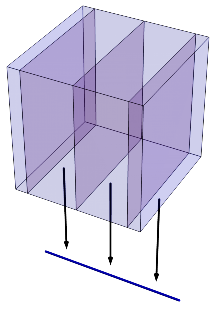
\includegraphics[width=\linewidth]{figures/linear-map-fibres.pdf}
}

\begin{Example}{爆破的纤维}\leavevmode\label{ex:fibres-of-affine-space-blowup}
令 $\pi:\operatorname{Bl}_{0}(\mathbb{A}^{n})\to\mathbb{A}^{n}$ 为爆破映射, 其中 $n>1$. 如上一节所述, $\mathbb{A}^{n}$ 中任意非零点上的纤维为单点, 而原点上的纤维同构于 $\mathbb{P}^{n-1}$. 由于 $\dim(\mathbb{A}^{n})=\dim(\operatorname{Bl}_{0}(\mathbb{A}^{n}))=n$ 且 $\pi$ 为满射, 预期纤维的维数为零. $\mathbb{A}^{n}$ 的每个非零点都符合这一预期, 但特殊点 $0$ 上的纤维的维数为 $n-1$, 大于预期.
\end{Example}

现在陈述纤维维数定理的第一部分, 它说明纤维绝不会比预期的小.

\begin{Theorem}{纤维维数定理, 第一部分}\leavevmode\label{thm:fiber-dimension-lower-bound}
令 $F:X\to Y$ 为拟射影簇之间的正则映射, 其中 $X$ 不可约. 则对任意 $b\in F(X)$, 都有
\[
  \dim(F^{-1}(b))\ge\dim(X)-\dim(\overline{F(X)}).
\]
\end{Theorem}

\BookPairedNoteLeft{
我们取 $F(X)\subseteq Y$ 的闭包, 因为 $F(X)$ 本身不一定是 $Y$ 的子簇. 见 Exercise~\ref{ex:image-of-affine-polynomial-map-not-quasiprojective}.
}{
如将看到的, Theorem~\ref{thm:fiber-dimension-lower-bound} 是维数论基本定理的一个推论. 下一个引理联系了这两个结果, 它实质上断言: 不可约拟射影簇的每一点都可局部用预期数量的方程定义.
}

\begin{Lemma}{$Y$ 中每一点都局部由 $\dim(Y)$ 个方程定义}\leavevmode\label{lem:point-locally-cut-out-by-dimension-many-functions}
若 $Y$ 是 $d$ 维不可约拟射影簇, $b\in Y$, 则存在仿射开子集 $U\subseteq Y$, 其中 $b\in U$, 以及正则函数 $F_{1},\ldots,F_{d}\in K[U]$, 使 $\mathcal{V}(F_{1},\ldots,F_{d})=\{b\}$.
\end{Lemma}
\begin{Proof}
若 $d=0$, 则 $Y=\{b\}$, $U=Y$ 满足所需结论. 故设 $d>0$. 先选取包含 $b$ 的仿射开子集 $V\subseteq Y$. 由于 $Y$ 不可约, $V$ 也不可约, 且 $\dim(V)=d>0$. 在同构意义下, 可以将 $V$ 表示为仿射空间的闭子集 $V\subseteq\mathbb{A}^{n}$. 我们将递归构造多项式 $g_{1},\ldots,g_{d}\in K[y_{1},\ldots,y_{n}]$, 都在 $b$ 处消没, 使 $V\cap\mathcal{V}(g_{1},\ldots,g_{k})$ 的每个不可约分支的维数为 $d-k$.

为开始递归, 选取 $g_{1}\in K[y_{1},\ldots,y_{n}]$, 使它在 $b$ 处消没, 但不在整个 $V$ 上消没 (例如, 若 $b'\in V\setminus\{b\}$ 与 $b$ 的第 $i$ 个坐标不同, 则多项式 $g_{1}=y_{i}-b_{i}$ 就可以). 由于 $V$ 是 $d$ 维不可约簇, 维数论基本定理推出 $V\cap\mathcal{V}(g_{1})$ 的每个不可约分支的维数为 $d-1$.

现假设已经找到 $g_{1},\ldots,g_{k}\in K[y_{1},\ldots,y_{n}]$, 它们都在 $b$ 处消没, 使 $V\cap\mathcal{V}(g_{1},\ldots,g_{k})$ 的每个不可约分支的维数为 $d-k>0$. 由 Exercise~\ref{ex:choose-polynomial-vanishing-at-point-not-on-components}, 可选取 $g_{k+1}\in K[y_{1},\ldots,y_{n}]$, 使它在 $b$ 处消没, 但不在 $V\cap\mathcal{V}(g_{1},\ldots,g_{k})$ 的任何整个不可约分支上消没. 再由维数论基本定理, $V\cap\mathcal{V}(g_{1},\ldots,g_{k},g_{k+1})$ 的每个不可约分支的维数为 $d-k-1$, 如所需.

由构造, $V\cap\mathcal{V}(g_{1},\ldots,g_{d})$ 是零维的, 因而是有限集 $\{b,b_{1},\ldots,b_{\ell}\}$. 令 $U\subseteq V$ 为任一包含于开集 $V\setminus\{b_{1},\ldots,b_{\ell}\}$ 中的 $b$ 的仿射开邻域, 对 $k=1,\ldots,d$ 置 $F_{k}=g_{k}|_{U}$. 则 $F_{1},\ldots,F_{d}$ 是 $U$ 上的正则函数, 且 $\mathcal{V}(F_{1},\ldots,F_{d})=\{b\}$, 证毕.
\end{Proof}

现在证明纤维维数定理的第一部分.

\begingroup
\renewcommand{\AJProofBegin}{%
  \par\addvspace{\topsep}\noindent
  {\sffamily\bfseries\CJKfamily{pffont}Proof of Theorem~\ref{thm:fiber-dimension-lower-bound}}\enspace\ignorespaces
}
\begin{Proof}
由于定理的陈述不涉及 $\overline{F(X)}$ 之外的 $Y$ 的部分, 可假设 $Y=\overline{F(X)}$. 于是 $F:X\to Y$ 为有稠密像的正则映射. $X$ 的不可约性蕴含 $Y$ 不可约 (Exercise~\ref{ex:image-and-closure-of-irreducible-space-are-irreducible}). 令 $b\in F(X)$, 置 $d=\dim(Y)$. 由 Lemma~\ref{lem:point-locally-cut-out-by-dimension-many-functions}, 选取仿射开子集 $U\subseteq Y$ 和正则函数 $F_{1},\ldots,F_{d}\in K[U]$, 使
\[
  \mathcal{V}(F_{1},\ldots,F_{d})=\{b\}.
\]
置 $V=F^{-1}(U)$, 由正则映射的连续性, 这是 $X$ 的一个开子簇. 由于 $X$ 不可约, $V$ 也不可约, 且 $\dim(V)=\dim(X)$. 用 $G:V\to U$ 表示 $F$ 在 $V$ 上的限制, 注意 $F^{-1}(b)=G^{-1}(b)$. 因为 $G(a)=b$ 当且仅当对所有 $i=1,\ldots,d$ 有 $F_{i}(G(a))=0$, 可得
\[
  G^{-1}(b)=\mathcal{V}(G^{*}(F_{1}),\ldots,G^{*}(F_{d})).
\]
由于 $G^{-1}(b)$ 是 $V$ 上 $d$ 个正则函数的消没集, Corollary~\ref{cor:dimension-bound-for-quasiprojective-vanishing-set} 蕴含
\[
  \dim(G^{-1}(b))\ge\dim(V)-d.
\]
由构造, 此不等式正是定理陈述中的断言:
\[
  \dim(F^{-1}(b))\ge\dim(X)-\dim(\overline{F(X)}).
\]
\end{Proof}
\endgroup

现在进入纤维维数定理的第二部分, 也是较难的一部分. 它实质上说明, 在像的某个非空开子集上, 纤维总能达到预期的维数.

\begin{Theorem}{纤维维数定理, 第二部分}\leavevmode\label{thm:fiber-dimension-equality-on-open-subset}
令 $F:X\to Y$ 为拟射影簇之间的正则映射, 其中 $X$ 不可约. 则存在非空开子集 $U\subseteq Y$, 使对每个 $b\in U$, 有 $F^{-1}(b)=\varnothing$, 或者
\[
  \dim(F^{-1}(b))=\dim(X)-\dim(\overline{F(X)}).
\]
\end{Theorem}
\begin{Proof}
如在 Theorem~\ref{thm:fiber-dimension-lower-bound} 的证明中, 假设 $Y=\overline{F(X)}$. 注意 $X$ 的不可约性于是蕴含 $Y$ 不可约. 现在归约到 $X,Y$ 都为仿射簇的情形.

\textbf{(归约到 $Y$ 为仿射簇)} 假设定理在陪域为仿射簇时成立. 令 $F:X\to Y$ 为正则映射, 其中 $X$ 不可约, 且 $\overline{F(X)}=Y$. 对任一非空仿射开集 $V\subseteq Y$, 可将假设应用于 $F$ 在 (开) 原像 $F^{-1}(V)\subseteq X$ 上的限制. 因此, 由假设, 存在非空开集 $U\subseteq V$, 使对所有 $b\in U$,
\[
  F^{-1}(b)=\varnothing\qquad\text{或}\qquad
  \dim(F^{-1}(b))=\dim(F^{-1}(V))-\dim(V).
\]
由于 $X,Y$ 不可约, $F^{-1}(V)\subseteq X$ 和 $V\subseteq Y$ 都是稠密开集, 因而它们的维数分别与 $X,Y$ 相同. 由此可知, 对所有 $b\in U$,
\[
  F^{-1}(b)=\varnothing\qquad\text{或}\qquad
  \dim(F^{-1}(b))=\dim(X)-\dim(Y).
\]
由于 $U$ 是开集 $V\subseteq Y$ 的非空开子集, 它也是 $Y$ 的非空开集. 由此证明, 所选的 $U$ 满足 $F:X\to Y$ 的定理结论. 既然定理的一般形式由陪域为仿射簇的特例推出, 以下假设 $Y$ 为仿射簇.

\textbf{(归约到 $X$ 为仿射簇)} 假设定理在定义域为仿射簇时成立. 令 $F:X\to Y$ 为正则映射, 其中 $X$ 不可约, 且 $\overline{F(X)}=Y$. 由 Theorem~\ref{thm:quasiprojective-varieties-have-finite-affine-open-covers}, 选取有限多个仿射开子集 $V_{1},\ldots,V_{k}\subseteq X$, 使 $X=V_{1}\cup\cdots\cup V_{k}$. 由于 $X$ 不可约, 每个 $V_{i}$ 都在 $X$ 中稠密, 从而 $F(V_{i})$ 在 $Y$ 中稠密 (Exercise~\ref{ex:continuous-map-with-dense-image-maps-dense-subsets-to-dense-subsets}). 令 $F_{i}:V_{i}\to Y$ 为 $F$ 在 $V_{i}$ 上的限制. 由于 $V_{i}$ 仿射且不可约, 又有 $\overline{F_{i}(V_{i})}=Y$, 我们的假设蕴含存在非空开子集 $U_{i}\subseteq Y$, 使对每个 $b\in U_{i}$,
\[
  \begin{aligned}
  F_{i}^{-1}(b)&=\varnothing\\
  \text{或}\qquad\dim(F_{i}^{-1}(b))&=\dim(V_{i})-\dim(Y)=\dim(X)-\dim(Y).
  \end{aligned}
\]
考察非空开集 $U=U_{1}\cap\cdots\cap U_{k}\subseteq Y$, 令 $b\in U$. 若 $Z$ 为 $F^{-1}(b)$ 的一个不可约分支, 则至少对一个 $i$ 有 $V_{i}\cap Z$ 非空, 因为 $X=V_{1}\cup\cdots\cup V_{k}$. 因此
\[
  \dim(Z)=\dim(V_{i}\cap Z)\le\dim(F_{i}^{-1}(b))=\dim(X)-\dim(Y).
\]
第一个等式来自 $Z$ 不可约这一假设, 它蕴含 $V_{i}\cap Z$ 稠密; 不等式来自 $V_{i}\cap Z\subseteq F_{i}^{-1}(b)$; 第二个等式来自 $b\in U_{i}$ 这一假设. 由于已经找到 $F^{-1}(b)$ 的每个不可约分支维数的一致上界, 可知 $\dim(F^{-1}(b))\le\dim(X)-\dim(Y)$. 另一个不等式由 Theorem~\ref{thm:fiber-dimension-lower-bound} 得到. 因此, 已构造非空开集 $U\subseteq Y$, 使对每个 $b\in U$,
\[
  F^{-1}(b)=\varnothing\qquad\text{或}\qquad
  \dim(F^{-1}(b))=\dim(X)-\dim(Y).
\]
既然定理的一般形式由定义域为仿射簇的情形推出, 以下假设 $X$ 为仿射簇.

\textbf{($X$ 和 $Y$ 为仿射簇的证明)} 令 $F:X\to Y$ 为不可约仿射簇之间的正则映射, 使 $\overline{F(X)}=Y$. 由于 $F(X)$ 在 $Y$ 中稠密, 拉回同态 $F^{*}:K[Y]\to K[X]$ 为单射 (Exercise~\ref{ex:density-dominance-and-injective-pullback}). 通过这一单射, 将 $K[Y]$ 视为 $K[X]$ 的子代数. 取分式域后, 也将 $K(Y)$ 视为 $K(X)$ 的子域. 关于超越次数, 有
\begin{equation}\label{eq:transcendence-degree-difference-for-fibres}
  \operatorname{trdeg}_{K(Y)}K(X)
  =\operatorname{trdeg}_{K}K(X)-\operatorname{trdeg}_{K}K(Y),
\end{equation}
因为 $K(Y)$ 在 $K$ 上的每个超越基都能扩充为 $K(X)$ 在 $K$ 上的超越基, 而扩充进去的元素给出 $K(X)$ 在 $K(Y)$ 上的一个超越基 (Exercise~\ref{ex:transcendence-degrees-add-in-tower}).

把 $X$ 写成仿射空间的闭子集 $X\subseteq\mathbb{A}^{m}$, 定义 $A\subseteq K(X)$ 为坐标函数 $[x_{1}],\ldots,[x_{m}]$ 生成的 $K(Y)$-代数:
\[
  A=K(Y)\bigl[[x_{1}],\ldots,[x_{m}]\bigr]\subseteq K(X).
\]
由于 $A$ 在 $K(Y)$ 上由 $[x_{1}],\ldots,[x_{m}]$ 有限生成, Noether 正规化定理保证存在有限的 Noether 基 $\{H_{1},\ldots,H_{e}\}\subseteq A$. 更具体地说, $H_{1},\ldots,H_{e}$ 是 $A$ 中在 $K(Y)$ 上代数独立的元素, 使 $A$ 在 $K(Y)[H_{1},\ldots,H_{e}]$ 上整. 特别地, 对每个 $i=1,\ldots,m$, 都存在首一多项式
\[
  g_{i}(z)\in\bigl(K(Y)[H_{1},\ldots,H_{e}]\bigr)[z],
\]
使 $g_{i}([x_{i}])=0\in A$. 由于 $K(X)=K([x_{1}],\ldots,[x_{m}])$, 且每个 $[x_{i}]$ 在 $K(Y)[H_{1},\ldots,H_{e}]$ 上代数, 可知 Noether 基 $\{H_{1},\ldots,H_{e}\}$ 给出 $K(X)$ 在 $K(Y)$ 上的一个超越基. 于是 \eqref{eq:transcendence-degree-difference-for-fibres} 蕴含
\[
  e=\dim(X)-\dim(Y).
\]
由 $A$ 的定义, 对每个 $i=1,\ldots,e$, 可对某些 $F_{i}\in K[X]$, $G_{i}\in K[Y]\setminus\{0\}$ 写 $H_{i}=F_{i}/G_{i}$. 此外, 把 $g_{i}(z)$ 看作 $H_{1},\ldots,H_{e},z$ 的多项式时, 它的每个系数都是 $K(Y)$ 的元素, 因而可以表示为 $Y$ 上正则函数的商. 令 $G\in K[Y]\setminus\{0\}$ 为 $G_{1},\ldots,G_{e}$ 和 $g_{1}(z),\ldots,g_{e}(z)$ 的系数中作为分母出现的所有 $Y$ 上正则函数的乘积, 定义非空开集
\[
  U=Y\setminus\mathcal{V}(G).
\]
现在论证 $U$ 满足定理的结论.

令 $b\in U$, 假设 $F^{-1}(b)\ne\varnothing$. $U$ 的构造意味着对所有 $i=1,\ldots,e$ 有 $G_{i}(b)\ne0$. 函数 $H_{i}=F_{i}/G_{i}$ 在纤维 $F^{-1}(b)$ 上的限制给出正则函数 $H_{i}^{b}\in K[F^{-1}(b)]$, 定义为
\[
  H_{i}^{b}(a)=\frac{F_{i}(a)}{G_{i}(a)}
  \qquad\text{对每个 }a\in F^{-1}(b).
\]
类似地, 由于 $g_{i}(z)$ 的所有系数在 $U$ 上都是良定义的函数, 可以把多项式 $g_{i}(z)$ 的所有系数限制到纤维 $F^{-1}(b)$, 得到多项式
\[
  g_{i}^{b}(z)\in K[H_{1}^{b},\ldots,H_{e}^{b}][z].
\]
重要的是, 由于 $g_{i}(z)$ 首一, $g_{i}^{b}(z)$ 也首一. 因为 $F^{-1}(b)$ 在闭集 $X\subseteq\mathbb{A}^{m}$ 中闭, 坐标函数 $[x_{1}],\ldots,[x_{m}]$ 生成 $K[F^{-1}(b)]$. 将关系 $g_{i}([x_{i}])=0$ 限制到纤维 $F^{-1}(b)$, 得到关系 $g_{i}^{b}([x_{i}])=0\in K[F^{-1}(b)]$, 说明每个坐标函数都在 $K[H_{1}^{b},\ldots,H_{e}^{b}]$ 上整. 因此, Theorem~\ref{thm:finite-generation-integrality} 蕴含 $K[F^{-1}(b)]$ 在 $K[H_{1}^{b},\ldots,H_{e}^{b}]$ 上整. 由 Corollary~\ref{cor:bounds-on-transcendence-degree} 的第~\ref{part:transcendence-degree-upper-bound}~项, 可知
\[
  \dim(F^{-1}(b))\le e=\dim(X)-\dim(Y).
\]
结合 Theorem~\ref{thm:fiber-dimension-lower-bound}, 可得
\[
  \dim(F^{-1}(b))=\dim(X)-\dim(Y),
\]
定理得证.
\end{Proof}

下一例简要说明上一证明所用的几个关键想法.

\begin{Example}{Theorem~\ref{thm:fiber-dimension-equality-on-open-subset} 的证明示例}\leavevmode\label{ex:fiber-dimension-equality-by-clearing-denominators}
考察 $X=\mathcal{V}(xy_{1}-y_{2})\subseteq\mathbb{A}^{3}$ 和 $Y=\mathbb{A}^{2}$, 令 $F:X\to\mathbb{A}^{2}$ 为由 $F(a,b_{1},b_{2})=(b_{1},b_{2})$ 定义的正则映射. 稍加思考 (Exercise~\ref{ex:fibres-of-projection-from-affine-graph}) 可知, $\overline{F(X)}=Y$, $\dim(X)=\dim(Y)=2$, $F(X)$ 的任意非零点上的纤维是一个点, 而 $(0,0)$ 上的纤维同构于 $\mathbb{A}^{1}$. 本例的目标是针对这一具体的仿射簇之间的映射, 逐步说明 Theorem~\ref{thm:fiber-dimension-equality-on-open-subset} 的证明细节, 最终构造非空开集 $U\subseteq Y$, 使 $F$ 在其上的非空纤维都有预期的维数零.

注意 $K(Y)=K(y_{1},y_{2})$, 而 Theorem~\ref{thm:fiber-dimension-equality-on-open-subset} 的证明中出现的代数 $A$ 是
\[
  A=K(y_{1},y_{2})\bigl[[x]\bigr]\subseteq K(X).
\]
空集是 $A$ 在 $K(y_{1},y_{2})$ 上的一个 Noether 基, 因为唯一的生成元 $[x]$ 是首一多项式
\[
  g(z)=z-\frac{y_{2}}{y_{1}}\in K(y_{1},y_{2})[z]
\]
的一个根; 这是因为 $xy_{1}-y_{2}\in\mathcal{I}(X)$. 仿照 Theorem~\ref{thm:fiber-dimension-equality-on-open-subset} 的证明, 令 $G\in K[Y]=K[y_{1},y_{2}]$ 为 Noether 基和首一多项式中出现的所有分母的乘积. 此处 $G=y_{1}$, 所以 $U=\mathbb{A}^{2}\setminus\mathcal{V}(y_{1})$. 因此对任意 $(b_{1},b_{2})\in U$, 都有 $b_{1}\ne0$; 对任意 $(a,b_{1},b_{2})\in F^{-1}(b_{1},b_{2})$, 都得到良定义的首一关系
\[
  0=g(a)=a-\frac{b_{2}}{b_{1}}.
\]
在本例中, 这个关系从 $(b_{1},b_{2})$ 唯一确定 $a$, 表明 $U$ 上的纤维的维数为零, 如所预期.
\end{Example}

本节的最后一个结果是纤维维数定理的一个应用, 它提供了一种验证簇不可约的有用方法.

\begin{Theorem}{等维不可约纤维 $\implies$ 不可约}\leavevmode\label{thm:projective-domain-irreducible-from-equidimensional-irreducible-fibres}
令 $F:X\to Y$ 为满的正则映射, 其中 $X$ 射影, $Y$ 不可约. 若对每个 $b\in Y$, $F^{-1}(b)$ 不可约且维数相同, 则 $X$ 不可约.
\end{Theorem}
\begin{Proof}
令 $X_{1},\ldots,X_{k}$ 为 $X$ 的不可约分支; 我们要证明对某个 $i$ 有 $X=X_{i}$. 令 $F_{i}:X_{i}\to Y$ 为 $F$ 在 $X_{i}$ 上的限制. 由于 $X$ 射影, Theorem~\ref{thm:regular-images-of-projective-varieties-are-closed} 蕴含 $F(X_{i})$ 对每个 $i$ 都在 $Y$ 中闭. 又因为 $F$ 是满射, 可推出
\[
  Y=F(X)=\bigcup_{i=1}^{k}F(X_{i}).
\]
注意 $Y$ 的不可约性意味着至少对一个 $i$ 有 $Y=F(X_{i})$. 对每个满足 $F(X_{i})=Y$ 的 $i$, Theorem~\ref{thm:fiber-dimension-equality-on-open-subset} 蕴含存在非空开集 $U_{i}\subseteq Y$, 使
\[
  \dim(F_{i}^{-1}(b))=\dim(X_{i})-\dim(Y)\qquad\text{对所有 }b\in U_{i}.
\]
对每个满足 $F(X_{i})\ne Y$ 的 $i$, 置 $U_{i}=Y\setminus F(X_{i})$. 令 $U=U_{1}\cap\cdots\cap U_{k}$, 它是 $Y$ 的非空开子集.

选取某个 $b_{0}\in U$. 则 $F^{-1}(b_{0})$ 的不可约性蕴含它包含于某个 $X_{i}$. 不妨设 $F^{-1}(b_{0})\subseteq X_{1}$, 故 $F^{-1}(b_{0})=F_{1}^{-1}(b_{0})$. 由 $U$ 的定义可知 $F_{1}$ 为满射, 且
\[
  \dim(F^{-1}(b_{0}))=\dim(F_{1}^{-1}(b_{0}))=\dim(X_{1})-\dim(Y).
\]
现任取 $b\in Y$. 由于 $F$ 的所有纤维维数相同,
\begin{equation}\label{eq:common-fibre-dimension-from-surjective-component}
  \dim(F^{-1}(b))=\dim(F^{-1}(b_{0}))=\dim(X_{1})-\dim(Y).
\end{equation}
此外, 由 Theorem~\ref{thm:fiber-dimension-lower-bound}, 有
\begin{equation}\label{eq:fibre-dimension-lower-bound-for-surjective-component}
  \dim(F_{1}^{-1}(b))\ge\dim(X_{1})-\dim(Y).
\end{equation}
结合 \eqref{eq:common-fibre-dimension-from-surjective-component} 和 \eqref{eq:fibre-dimension-lower-bound-for-surjective-component}, 得 $\dim(F^{-1}(b))\le\dim(F_{1}^{-1}(b))$. 不过, 由于 $F_{1}^{-1}(b)\subseteq F^{-1}(b)$, 也得到反向不等式, 因而 $\dim(F_{1}^{-1}(b))=\dim(F^{-1}(b))$. 由假设 $F^{-1}(b)$ 不可约, 且 $F_{1}^{-1}(b)=F^{-1}(b)\cap X_{1}$ 是 $F^{-1}(b)$ 的同维闭子集, 可知 (Exercise~\ref{ex:quasiprojective-dimension-monotone-and-strict-for-proper-closed-subvariety}) $F^{-1}(b)=F_{1}^{-1}(b)$. 由于这对所有 $b\in Y$ 成立, 得 $X=X_{1}$, 如所需.
\end{Proof}

\BookExerciseHeading
\begin{BookExercises}
  \item\label{ex:image-of-affine-polynomial-map-not-quasiprojective} 令 $F:\mathbb{A}^{2}\to\mathbb{A}^{2}$ 由 $F(a_{1},a_{2})=(a_{1},a_{1}a_{2})$ 定义.
  \begin{enumerate}
    \item 计算 $F(\mathbb{A}^{2})\subseteq\mathbb{A}^{2}$.
    \item 证明 $F(\mathbb{A}^{2})$ 不是 $\mathbb{A}^{2}$ 的子簇.
    \item 对任意 $(b_{1},b_{2})\in\mathbb{A}^{2}$, 计算纤维 $F^{-1}(b_{1},b_{2})$.
  \end{enumerate}
  \item\label{ex:choose-polynomial-vanishing-at-point-not-on-components}
  \begin{enumerate}
    \item 令 $a_{0},a_{1},\ldots,a_{k}\subseteq\mathbb{A}^{n}$ 为 $\mathbb{A}^{n}$ 中互不相同的点. 证明存在 $f\in K[x_{1},\ldots,x_{n}]$, 使 $f(a_{i})=0$ 当且仅当 $i=0$.
    \item 令 $a\in\mathbb{A}^{n}$, $X_{1},\ldots,X_{k}\subseteq\mathbb{A}^{n}$ 为非空子集, 没有一个等于 $\{a\}$. 证明存在 $f\in K[x_{1},\ldots,x_{n}]$, 使 $f(a)=0$, 且对所有 $i=1,\ldots,k$ 有 $f\notin\mathcal{I}(X_{i})$.
  \end{enumerate}
  \item\label{ex:image-and-closure-of-irreducible-space-are-irreducible} 令 $F:X\to Y$ 为拓扑空间之间的连续映射, $X$ 不可约. 证明 $F(X)$ 和 $\overline{F(X)}$ 都是 $Y$ 的不可约子空间.
  \item\label{ex:continuous-map-with-dense-image-maps-dense-subsets-to-dense-subsets} 设 $F:X\to Y$ 为拓扑空间之间的连续映射, 使 $F(X)$ 在 $Y$ 中稠密. 证明若 $U$ 在 $X$ 中稠密, 则 $F(U)$ 在 $Y$ 中稠密.
  \item\label{ex:transcendence-degrees-add-in-tower} 令 $K\subseteq L\subseteq M$ 为域, 使 $L$ 在 $K$ 上有限生成, $M$ 在 $L$ 上有限生成. 证明
  \[
    \operatorname{trdeg}_{K}(M)
    =\operatorname{trdeg}_{K}(L)+\operatorname{trdeg}_{L}(M).
  \]
  \item\label{ex:fibres-of-projection-from-affine-graph} 置 $X=\mathcal{V}(xy_{1}-y_{2})\subseteq\mathbb{A}^{3}$ 和 $Y=\mathbb{A}^{2}$, 令 $F:X\to\mathbb{A}^{2}$ 为由 $F(a,b_{1},b_{2})=(b_{1},b_{2})$ 定义的正则映射.
  \begin{enumerate}
    \item 证明 $\overline{F(X)}=Y$.
    \item 证明 $\dim(X)=\dim(Y)=2$.
    \item 证明 $F$ 在 $\mathbb{A}^{2}$ 的任意非零点上的纤维或者为空, 或者为单点.
    \item 证明 $F^{-1}(0,0)$ 同构于 $\mathbb{A}^{1}$.
  \end{enumerate}
  \item\label{ex:fibre-dimension-sets-closed-for-projective-maps} 令 $F:X\to Y$ 为射影簇之间的满的正则映射. 证明集合
  \[
    Y_{k}=\{b\in Y\mid\dim(F^{-1}(b))\ge k\}
  \]
  在 $Y$ 中闭.
\end{BookExercises}

\par\medskip
{\footnotesize
\noindent\textbf{开放获取.} 本章按照
\href{http://creativecommons.org/licenses/by-nc/4.0/}{Creative Commons Attribution-NonCommercial 4.0 International License}
的条款授权. 该许可允许以任何媒介或格式进行非商业性使用, 分享, 改编, 分发和复制, 但须对原作者和来源作适当署名, 提供 Creative Commons 许可的链接, 并说明是否作了修改.

\noindent
\begin{minipage}[t]{.17\linewidth}
  \vspace{0pt}
\includegraphics[width=.9\linewidth]{figures/source-cc-by-nc.png}
\end{minipage}\hfill
\begin{minipage}[t]{.81\linewidth}
  \vspace{0pt}本章的图片或其他第三方材料均纳入本章的 Creative Commons 许可, 除非材料的署名行另有注明. 如果材料未纳入本章的 Creative Commons 许可, 且您拟进行的使用未获法律规定的许可或超出允许使用的范围, 则须直接向著作权持有人取得许可.
\end{minipage}\par}
